\documentclass{article}
\usepackage{blindtext}
\usepackage{titlesec}
%\usepackage[utf8]{inputenc}
\usepackage{listings}
\usepackage{amsmath}
\usepackage{graphics}
\usepackage{amssymb} 
\usepackage{amsthm}
\usepackage{graphicx}
\usepackage{hyperref}
\usepackage{biblatex}
\usepackage{xcolor}
\usepackage{fancyhdr}
\usepackage{float}

\hypersetup{                    % parametrage des hyperliens
    colorlinks=true,                % colorise les liens
    breaklinks=true,                % permet les retours à la ligne pour les liens trop longs
    urlcolor= true,                 % couleur des hyperliens
    linkcolor= true,                % couleur des liens internes aux documents (index, figures, tableaux, equations,...)
    citecolor= true,              % couleur des liens vers les references bibliographiques
    }

\begin{document}
\begin{titlepage}
\begin{figure} 

\includegraphics[width=0.4\textwidth]{images/cnrslogo.jpeg}

\includegraphics[width=0.4\textwidth]{images/inria.png}
    \centering
\end{figure}

\centering
\title{}\author{}\date{}
\centering
\vspace{3cm}
{\bfseries\LARGE CNRS Alsace delegation - INRIA \par}
\vspace{4cm}
{\bfseries\LARGE Training augmented interpolation \par}
\vspace{1cm}
{\Large FONSECA HINCAPIÉ Diana Sol Angel\par}
\vspace{1cm}
{\Large STAGE M1 CSMI \par}
\vspace{3cm}
{\Large Supervisor: \par}
\vspace{0.5cm}
{\Large M.FRANCK Emmanuel\par}
\vspace{0.5cm}
{\Large M.NAVORET Laurent\par}
\end{titlepage}


%Table of contents
\maketitle
\tableofcontents 
\newpage






\section{Introduction}

\section{Objectives}
The main objective of this internship was to 


\section{Theoretical Framework}


\subsection{Augmented Interpolation}

\subsubsection{Deep Lagrange Interpolation}
The deep Lagrange interpolation operator is definded as follows:
\begin{equation*}
    \mathcal{I}_d^m(f)=\sum_{i=1}^n \frac{f\left(x_i\right)}{u_{\theta_i}\left(x_i\right)} P_i(x) u_{\theta_i}(x)
\end{equation*}

with $P_i\left(x_j\right)=\delta_{i j}$

Using this choice, we obtain that $\mathcal{I}_d(f)\left(x_i\right)=f\left(x_i\right)$ as the classical Lagrange interpolation operator. 

\subsubsection{Deep Lagrange interpolation with PINNs}

We will consider a specific case of the deep interpolation:
$$
\mathcal{I}_d^m(f)=\sum_{i=1}^n \frac{f\left(x_i\right)}{u_\theta\left(x_i\right)} P_i(x) u_\theta(x)=\mathcal{I}^m\left(\frac{f}{u_\theta}\right) u_\theta(x)
$$
This interpolation will be better than the classical one if $\frac{f}{u_\theta} \approx=1$ since we have the following error on the interpolation:
$$
\left\|f-\mathcal{I}_d^m(f)\right\|_{H^m} \leq C h^{m+1}\left\|\left(\frac{f}{u_\theta}\right)^{\prime \prime}\right\|_{L^2}\|f\|_{H^m}
$$

Now we the question is how choose $u_\theta(x)$. We propose to use a neural network which will approximate the $u_\theta(x)$ function. 

$$
u_\theta\left(x ; t, \mu, a(x), a^{\prime}(x)\right)
$$

We will train these neural networks with a P \textit{Physics Informed Neural Network} strategy and we will use the previous interpolation to approximate the solution of the PDE.

\subsection{Supervised and unsupervised learning}

\subsubsection{Supervised learning}

Supervised learning is a subcategory of machine learning and artificial intelligence. 
It is defined by its use of labeled datasets to train algorithms that to classify data or predict outcomes accurately. As input data is fed into the model, 
it adjusts its weights until the model has been fitted appropriately, which occurs as part of the cross validation process. Supervised learning uses a training set to teach models to yield the desired output. This training dataset includes inputs and correct outputs, which allow the model to learn over time. The algorithm measures its accuracy through the loss function, 
adjusting until the error has been sufficiently minimized. 

\subsubsection{Unsupervised learning}
Unsupervised learning uses machine learning algorithms to analyze and cluster unlabeled datasets. These algorithms discover hidden patterns or data groupings without the need for human intervention. Its ability to discover similarities and differences in information make it the ideal solution for exploratory data analysis, cross-selling strategies, customer segmentation, and image recognition.


In our context we will be interested in both supervised and unsupervised learning. We will use supervised learning to train the neural networks without knowing the solution and unsupervised learning to learn from the data calculated based on the exact solution of the PDE.

\subsection{Neural Networks}

Neural networks process training data by mimicking the interconnectivity of the human brain through layers of nodes, each node is made up of inputs, weights, a bias (or threshold), and an output. If that output value exceeds a given threshold, it “fires” or activates the node, passing data to the next layer in the network. Neural networks learn this mapping function through supervised learning,
adjusting based on the loss function through the process of gradient descent. When the cost function is at or near zero, we can be confident in the model’s accuracy to yield the correct answer.

They are basically functions that map an input $X$ to an output $Y$ by performing successive linear and nonlinear transformations. The linear transformations are represented by a set of weights $W$ and biases $b$ and the nonlinear transformations are represented by activation functions $\sigma$. The output of a neural network is given by:

$$\overline{u_\theta}(X)=W_n\sigma_{n-1}(W_{n-1}\sigma_{n-2}(...(W_2(W_1X+b_1)+b_2)+..)+b_{n-1})+b_n$$

\begin{figure}[H]
    \centering
    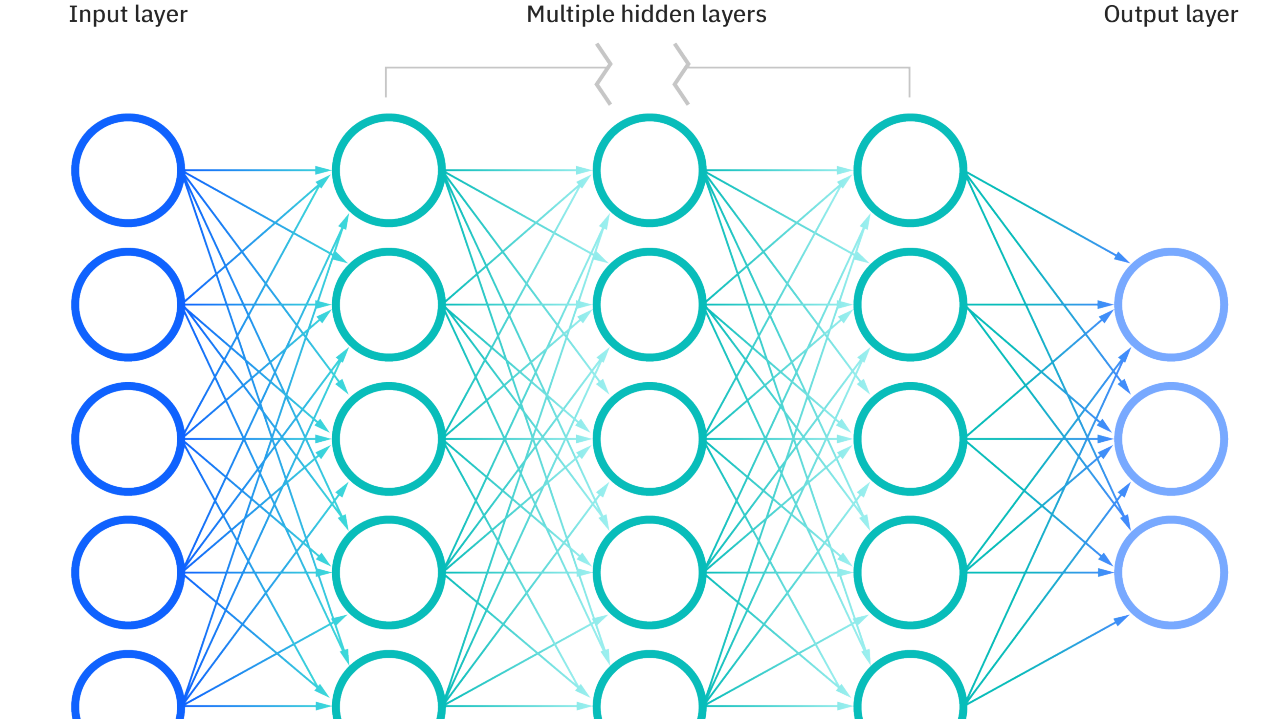
\includegraphics[width=0.5\textwidth]{images/neural_network.png}
    \caption{Neural Network Architecture}
\end{figure}
%Ajouter plus après
\subsection{Physics Informed Neural Networks}

PINNs are a scientific machine learning technique used to solve problems in our case involving Partial Differential Equations (PDEs), they approximate PDE solutions by training a neural network to minimize a loss function; it includes terms reflecting the initial and boundary conditions along the space-time domain’s boundary and the PDE residual at selected points in the domain (called collocation point). 
they are deep-learning networks that, given an input point in the integration domain, produce an estimated solution in that point of a differential equation after training. Incorporating a residual network that encodes the governing physics equations is a significant novelty with PINNs. 
The basic concept behind PINN training is that it can be thought of as an unsupervised strategy that does not require labelled data, such as results from prior simulations or experiments.
It works by integrating the mathematical model into the network and reinforcing the loss function with a residual term from the governing equation, which acts as a penalizing term to restrict the space of acceptable solutions.

PINN can be viewed as an unsupervised learning approach when they are trained solely using physical equations and boundary conditions for forward problems; however, for inverse problems or when some physical properties are derived from data that may be noisy, PINN can be considered supervised learning when they are trained using the data from the calculation of the exact solution of the PDE.
\begin{figure}[H]
    \centering
    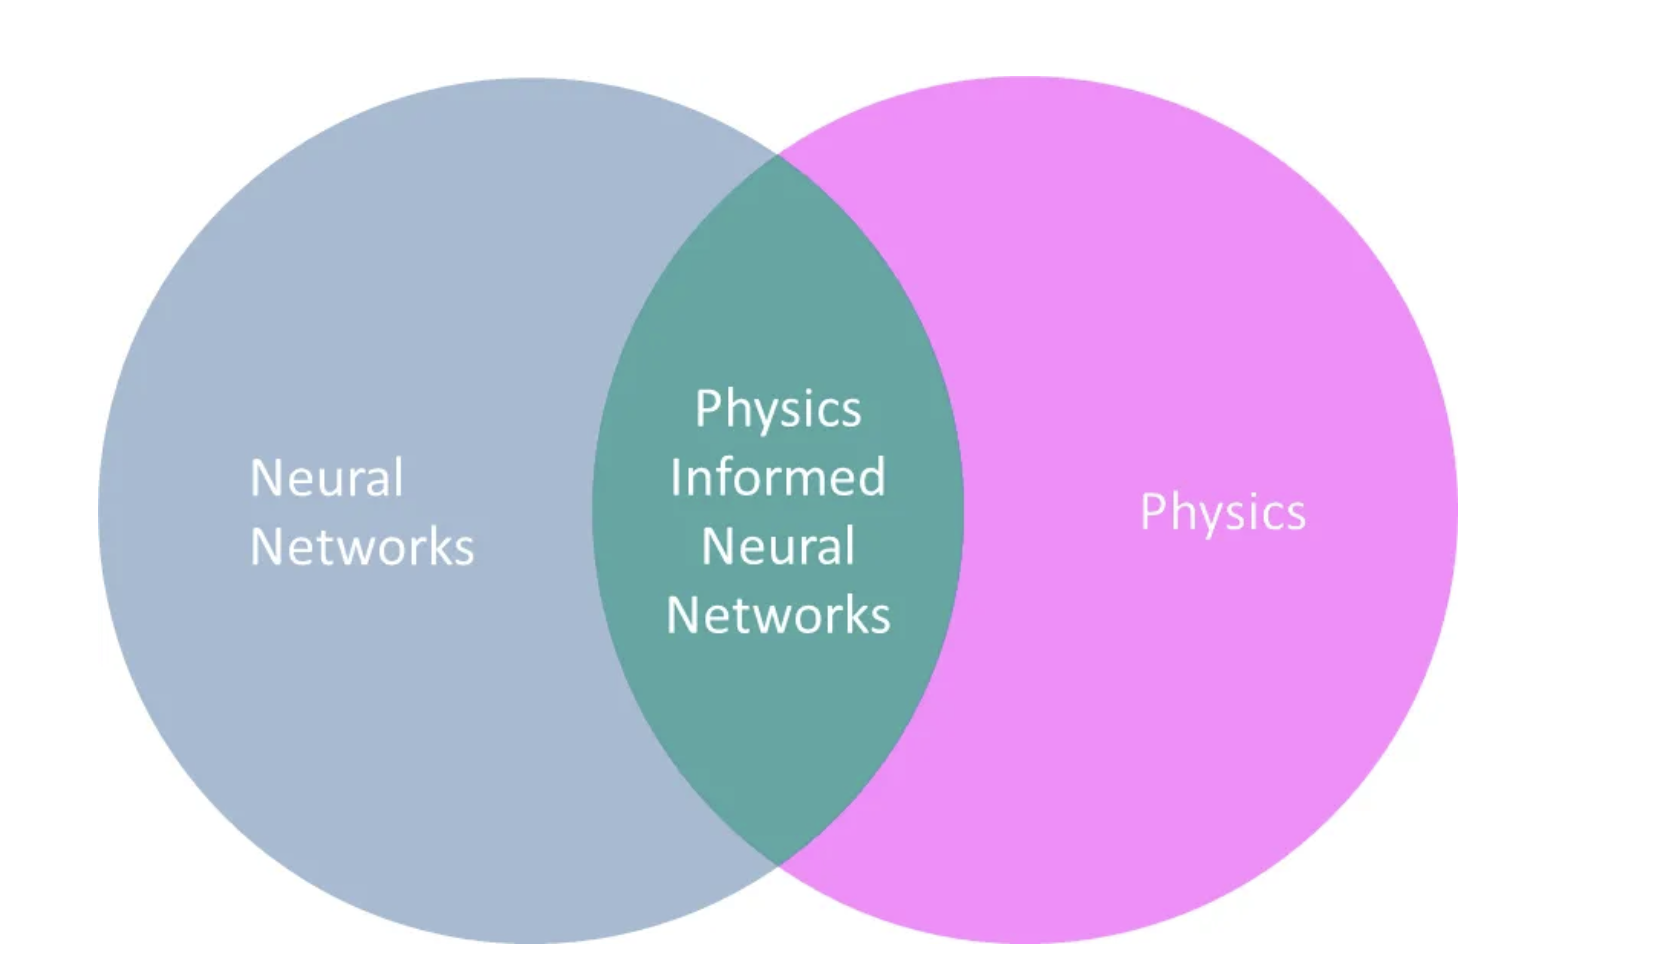
\includegraphics[width=0.5\textwidth]{images/pinns}
    \caption{PINNs}
\end{figure}

\subsubsection{Architecture of PINNs}

PINN are composed of three components: a neural network, a physics-informed network, and a feedback mechanism. The first block is a NN, $u_θ$,
that accepts vector variables  and outputs the filed value u. The second block can be thought of PINN’s functional component, as it computes the derivative to determine the losses of equation terms,
as well as the terms of the initial and boundary conditions of the PDE. Generally, the first two blocks are linked using algorithmic differentiation, which is used to inject physical equations into 
the NN during the training phase. Thus, the feedback mechanism minimizes the loss according to some learning rate, in order to fix the NN parameters vector θ of the NN $u_θ$.
In the following, it will be clear from the context to what network we are referring to, whether the NN or the functional network that derives the physical information.

%ajouter une fois que j'ai la bonne architecture qu'on va utiliser pour le PINN
% \begin{figure}[H]
%     \centering
%     \includegraphics[width=0.5\textwidth]{images/archpinns.png}
%     \caption{PINNs}
% \end{figure}


\subsubsection{Universal Approximation Theorem}

The representational ability of neural networks is well established. According to the universal approximation theorem:
The universal approximation theorem states that any continuous function  $$f : [0, 1]n \rightarrow [0, 1]$$  can be approximated arbitrarily well by a neural network with at least 1 hidden layer with a finite number of weights.
Even if neural networks can express very complex functions compactly, determining the precise parameters (weights and biases) required to solve a specific PDE can be difficult.



% \subsubsection{Training PINNs} AUN NO SEGURO  SI poner esta parte 
\subsubsection{Feed-forward Neural Network}


% \subsubsection{Loss Function}
\subsubsection{Error Estimation}
%explain the monte carlo approach (4:51video )


\subsubsection{PINNs for solving PDEs} 


In this project we were particularly interested in approximate the $u\theta$ function, which is the solution of the following PDE:

\begin{equation*}
    \begin{cases}
    \frac{\partial u}{\partial t} + a \frac{\partial u\theta}{\partial x} = 0 \quad (x,t) \in \Omega \times (0,T] \\
    u\theta(x,t=0) = u_0(x) \quad x \in \delta \Omega \\
    \end{cases}
\end{equation*}

Where $a$ is a constant that represents the velocity.

%25
%describir el proceso de como se utilizan las redes d eneuronas para poder resolver especialmente esta ecuacion diferencial parcial
%y como se puede utilizar para poder encontrar la solucion de la ecuacion diferencial parcial
We will train a neural network to approximate the solution of the PDE, we can do this by minimizing the error of the PDE in a certain number of points inside our domain.

We are going to represent our neural network by $overline{u_\theta}$  



\section{Implementation}
%Description of the code implementation with some code snippets and explanations of the most important parts of the code.


\section{Results}
\subsection{Finding $u\theta$ using PINNs}


\subsubsection{Unsupervised learning}


\subsubsection{Supervised learning}


\subsection{Solving using deep interpolation}



\section{Conclusions}


\section{Bibliography}
\bibitem[label]{1} {Scientific Machine Learning Through Physics–Informed Neural Networks: Where we are and What’s Next}
Salvatore Cuomo1 · Vincenzo Schiano Di Cola2 · Fabio Giampaolo1 · Gianluigi Rozza3 · Maziar Raissi4 · Francesco Piccialli1
26 July 2022
\bibitem[label]{2} {Supervised vs. Unsupervised Learning: What’s the Difference?} {https://www.ibm.com/cloud/blog/supervised-vs-unsupervised-learning}
\bibiitem[label]{3} {What are neural networks?} {https://www.ibm.com/topics/neural-networks}
\end{document}